\subsection{UDA by Backpropagation}

The purpose of the article "Unsupervised Domain Adaptation by Backpropagation" written by Yaroslav Ganin and Victor Lempitsky \cite{ganin2015unsupervised} is to tackle the problem of domain shift in machine learning and to propose a solution to this problem using a neural-network model with few standard layers and gradient reversal layer (GRL). The GRL makes the network to learn domain-invariant features by minimizing the difference between the distributions of the source and target domains. The architecture of the model is shown below (see Figure \ref{fig: uda_back})

\begin{figure}[H]
    \centering
    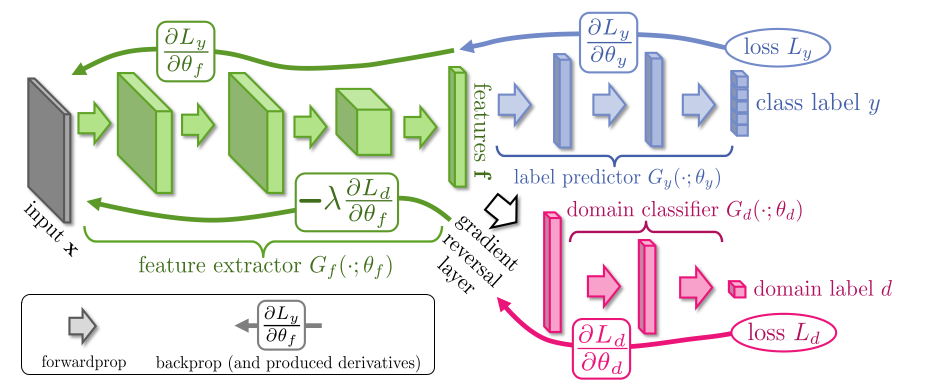
\includegraphics[width=0.8\textwidth]{Figures/From articles/uda_backpropagation.png}
    \caption{The proposed architecture includes a deep feature extractor (shown in green), a deep label predictor (shown in blue) and a domain classifier (shown in red). The domain classifier is connected to the feature extractor via a gradient reversal layer, which multiplies the incoming gradient by a negative constant during backpropagation-based training. The gradient reversal layer ensures that the feature distributions over the two domains become as similar as possible (i.e., indistinguishable by the domain classifier), resulting in domain-invariant features.}
    \label{fig: uda_back}
\end{figure}

The authors introduce an architecture that predicts both the label $y \in Y$ and the domain label $d \in \{0, 1\}$ for each input $\textbf{x}$. The architecture consists of three parts: feature extractor $\bold{f} = G_f(\textbf{x}, \theta_f)$, where $\theta_f$ is a vector that represents the parameters of all its layers; label predictor $G_y$ that maps the features obtained after feature extractor to the label $y$, with $\theta_y$ representing its parameters; domain classifier $G_d$ maps the same feature vector $\bold{f}$ to the domain label $d$, with $\theta_d$ representing its parameters. The purpose to minimize the label prediction loss for the source domain and simultaneously make the features $\textbf{f}$ invariant to the domain. To achieve this, the authors optimize the parameters $\theta_f$ of the feature mapping to maximize the loss of the domain classifier, however the parameters $\theta_d$ are optimized to minimize the loss of the domain classifier. The authors consider the loss

\begin{equation}
\begin{split}
E(\theta_f, \theta_y, \theta_d) & = \sum_{\substack{i=1..N \\ d_i = 0}} L_y(G_y(G_f(\textbf{x}_i; \theta_f); \theta_y), y_i) - \lambda \sum_{i = 1..N} L_d(G_d(G_f(\textbf{x}_i; \theta_f); \theta_d), y_i) \\ & = \sum_{\substack{i=0..N \\ d_i = 0}} L_y^i(\theta_f, \theta_y) - \lambda \sum_{i=1..N} L_d^i(\theta_f, \theta_d)
\end{split}
\end{equation} 

 where $L_y$ and $L_d$ are label prediction and domain classification losses, respectively. (index $i$ means the i-th example). It is considered the parameters $\hat{\theta}_f, \hat{\theta}_y, \hat{\theta}_d$ to gain a saddle point

\begin{equation}
\begin{split}
(\hat{\theta}_f , \hat{\theta}_y ) = \arg \min_{\theta_f, \theta_y} E(\theta_f, \theta_y, \hat{\theta}_d)
\\
\hat{\theta}_d = \arg \max_{\theta_d} E(\hat{\theta}_f, \hat{\theta}_y, \theta_d)
\end{split}
\end{equation}

During learning, the trade-off between the two objectives that shape the features is controlled by the parameter $\lambda$. The following stochastic updates can find a saddle point

\begin{equation}
\begin{split}
\theta_f & \leftarrow \theta_f - \mu \left( \dfrac{\partial L_y^i}{\partial \theta_f} - \lambda \dfrac{\partial L_d^i}{\partial \theta_f} \right) \\ 
\theta_y & \leftarrow \theta_y - \mu \dfrac{\partial L_y^i}{\partial \theta_y} \\ 
\theta_d & \leftarrow \theta_d - \mu \dfrac{\partial L_d^i}{\partial \theta_d} 
\end{split}
\end{equation} 

where $\mu$ is a learning rate. These updates are similar to SGD but with a $-\lambda$ factor in the first update to prevent dissimilar features across domains. Therefore, the authors introduce a GRL that acts as an identity transform during forward propagation but multiplies the gradient by $-\lambda$ during backpropagation.